%----------------------------------------
% Write your notes here
%----------------------------------------

\section{Problems of Experiments}
Random assignment is the “gold standard” for causal inference, but it has some limitations:\newline
1. Small sample size\newline
2. Researcher’s degree of freedom\newline
3. Publication bias: only those who reach statistically significant could be published.\newline
4. P hacking\newline 
\newline 
Factors influence power: \newline
N = sample size\newline
Alpha = significance level\newline  
Effect size (how strong is the effect? i.e. Cohen's D)\newline
P(significance | no effect) = "False Alarm"\newline
Power = 1- Beta = chance of detecting a real effect if one exists.\newline 
P(significance | effect) = "Hit"\newline
\newline
How to explain 95 percent confidence level: \newline
if we replicate the “experiments” infinite time, 95 percent results would contain the parameter (true value). 
\newline
\newline


\section{Caveat and Limitations}
1.randomization often is not feasible or ethical\newline
2.experiments are costly in terms of time and money\newline
3.it’s difficult to create convincing parallel worlds\newline
4.inevitably people deviate from their random assignment\newline
\newline

\section{Natural Experiments}
Sometimes we get lucky and nature effectively runs experiments for us e.g.:\newline
1. As-if random: people are randomly exposed to water sources\newline
2. Instrumental variables: a lottery influences military services:\newline
 IV influences treatment, but no association with the errors.\newline
3. Regression-discontinuities:\newline
 idea: things change around an arbitrary chosen threshold.\newline
4. Difference in differences:\newline
idea: compare difference after a sudden change with trends in a control group\newline
\newline
T C : “Compliers”\newline
T T : “Always treats”\newline
C C : “Never treats”\newline
\newline
ATE = pcATEc + paATEa + pnATEn\newline
\newline
(Fraction accept treatment in treatment group) – (Fraction accept treatment in control group) = (Pc + Pa) – Pa = Pc \newline
\newline

\section{Natural Experiments’ limitations}
1. Good natural experiments are hard to find\newline
2. They rely on naturally-occurring event rather than controlled manipulation\newline
3. Difficult to control for possible alternative explanations\newline
4. Limited sample size\newline
\newline
\newline


\begin{figure}[ht]
  \begin{center}
    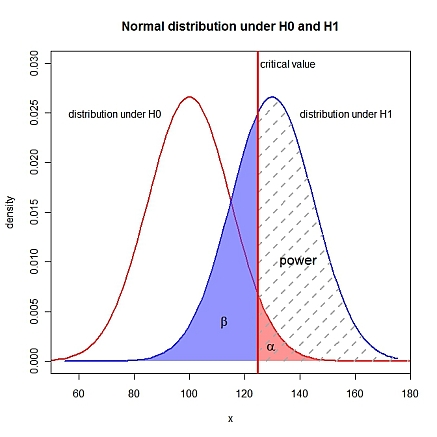
\includegraphics[width=0.5\textwidth]{rxoDS.jpg}
    \caption{
      This figure's source is as below: \newline http://jamescaldwell.info/optimization/the-maths-behind-statistically-significant-sample-sizes/.}
    \label{figure 1}
  \end{center}
\end{figure}


\begin{figure}[ht]
  \begin{center}
    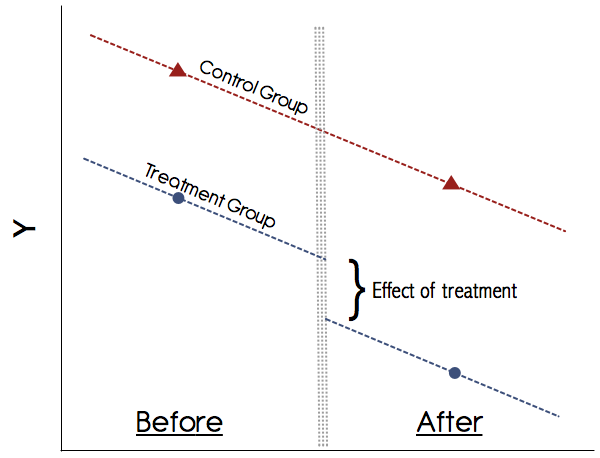
\includegraphics[width=0.5\textwidth]{J7P3p.png}
        \caption{Example plot for Difference in Differences.\newline  source: https://i.stack.imgur.com/J7P3p.png}
    \label{figure 2}
  \end{center}
\end{figure}


% ^.
\begin{figure}[ht]
  \begin{center}
    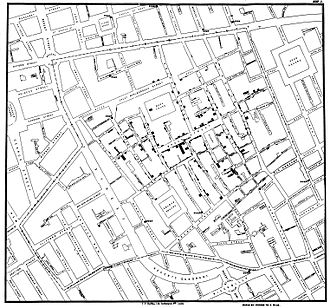
\includegraphics[width=0.5\textwidth]{330px-Snow-cholera-map-1.jpg}
        \caption{Example plot for natural experiment.\newline  source:  http://thelancet.com/journals/lancet/article/PIIS0140-6736(13)60830-2/fulltext?rss}
    \label{figure 3}
  \end{center}
\end{figure}
